%! Author = adnansiddiquei
%! Date = 04/06/2024

\section{Results}\label{sec:results}
To assess and demonstrate the performance of our AstroCLIP model, we reproduce a subset of the downstream tasks from
the original implementation by ~\cite{astroclip}.
The models with the lowest validation loss for each embedding dimensionality (as shown in Figure~\eqref{fig:val_loss})
were selected for evaluation.
The held-out validation set (composing of 39,599 of the 197,976 image-spectra pairs) was used to evaluate the performance
by assessing the accuracy of zero-shot k-NN redshift estimations and qualitative similarity retrieval tasks.
Notation used in this section intentionally follows that of the original paper for the reader's convenience.

\subsection{Zero-shot k-NN Redshift Estimation}\label{subsec:results-redshift-regression}

\begin{figure}[t]
    \centering
    \makebox[\textwidth]{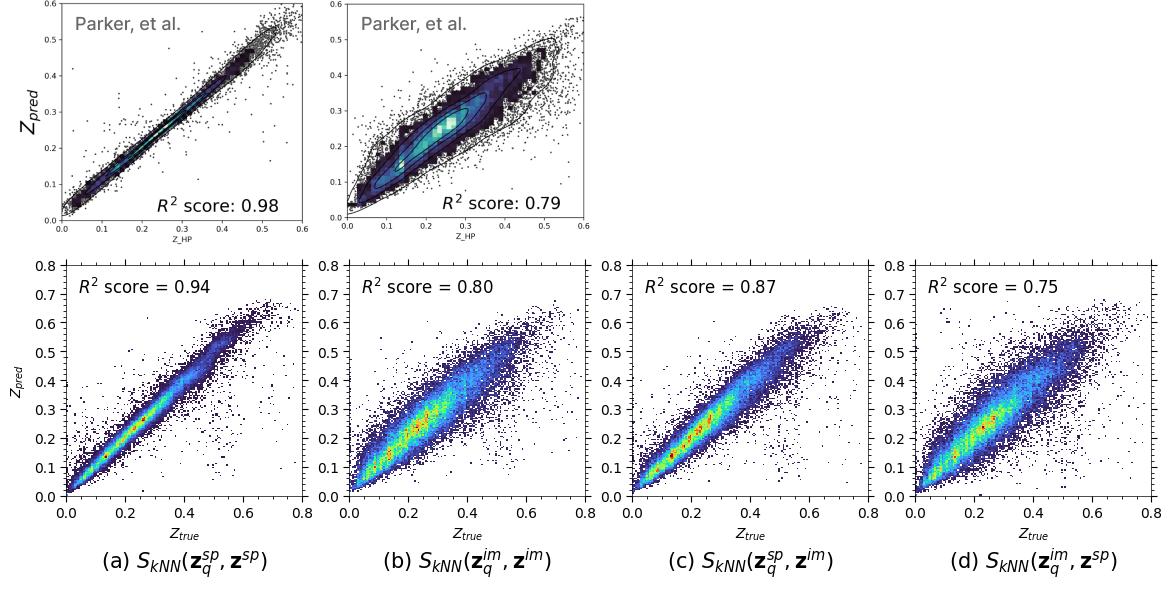
\includegraphics[width=1\textwidth]{figures/redshift_knn_regression_parker}}
    \caption{k-NN regression for zero-shot redshift prediction, showing predicted vs. true redshift.
    Top row is results from \cite{astroclip} for their 512-dim embedding model, bottom row is results from our 128-dim embedding
    model.
    $S_{kNN}(\mathbf{z}_{q}^{sp}, \mathbf{z}^{im})$ indicates the cross-modal prediction type where a spectrums redshift was
    predicted using its 16 closest embeddings derived from galaxy images.}
    \label{fig:rkr}
\end{figure}

\begin{figure}[t]
    \centering
    \makebox[\textwidth]{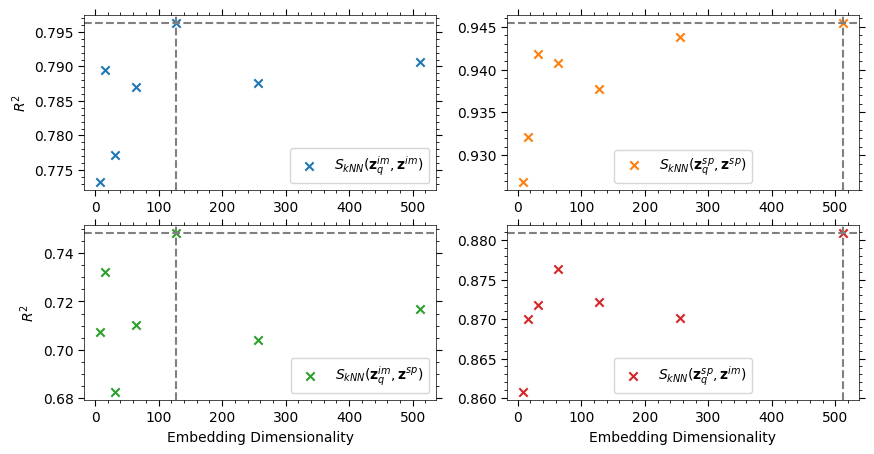
\includegraphics[width=1\textwidth]{figures/r2_vs_embedding_dim}}
    \caption{Consolidated results for all embedding dimensions and prediction types, displaying $R^{2}$ values vs. embedding dimensionality.
    These are the $R^{2}$ values derived if Figure~\eqref{fig:rkr} were plotted for all embedding dimensionalities.}
    \label{fig:r2_vs_embedding_dim}
\end{figure}

Figure~\eqref{fig:rkr} shows the zero-shot redshift predictions using k-NN regression on the learned embeddings for
the best 128-dimensional embedding model, and compares this to the 512-dimensional results from~\cite{astroclip}.
Our 128-dim image embedder outperforms the 512-dim image embedder from~\cite{astroclip} in the photometric redshift
prediction task (across a larger range in redshift values) with an $R^{2}$ value of 0.80 compared to their 0.79;
but falls short in the spectroscopic redshift prediction task with an $R^{2}$ value of 0.94 compared to their 0.98.
Figure~\eqref{fig:r2_vs_embedding_dim} then shows this same data in a more succinct manner for all embedding dimensionalities.
For a like-by-like comparison to~\cite{astroclip}, our 512-dim embedding performs marginally worse in the photometric redshift prediction
task with an $R^{2}$ value of 0.79, and marginally better in the spectroscopic redshift prediction task with an $R^{2}$ value
of 0.95.
These results demonstrate strong evidence that our AstroCLIP model is able to learn a meaningful representation of the
data, as the redshift predictions are highly correlated with the true redshift values.
More interestingly, our results show that even low-dimensional embeddings are able to perform well in the zero-shot
redshift prediction task, with the 8-dim and 16-dim embeddings generally performing at a similar level to the higher
dimensional embeddings across all prediction types.

Architecturally, these results indicates that the vision transformer architecture used by~\cite{astroclip} gave no
significant advantage over the 2D convolutional architecture used in this work for the image embedder.
However, the transformer architecture used for the spectrum embedder by~\cite{astroclip} outperformed the 1D convolutional
architecture used in this work for the spectrum embedder, and adds promise to the potential of transformer architectures
for spectral data.

\subsection{Retrieval by Cosine Similarity}\label{subsec:results-retrieval}
\begin{figure}[t]
    \centering
    \makebox[\textwidth]{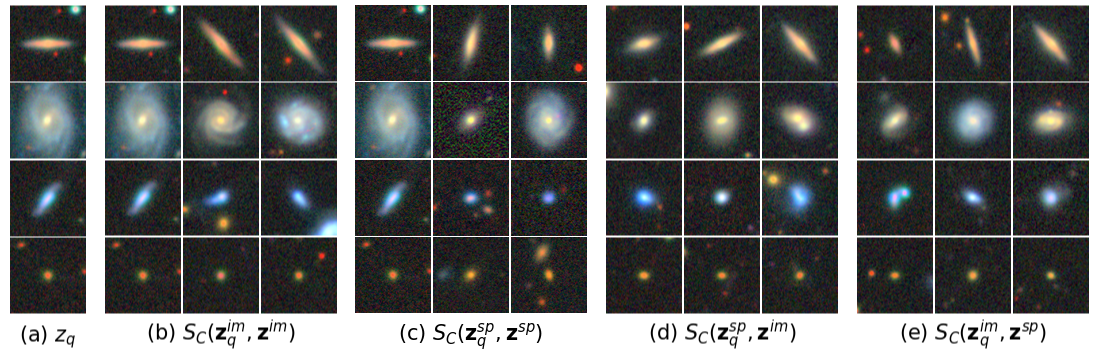
\includegraphics[width=1\textwidth]{figures/sim_search_images_all}}
    \caption{Cosine similarity search results using the 128-dimensional model. (a) 4 Query galaxies;
        (b, c, d, e) Top 3 similar galaxies across the 4 prediction types.
        By construction, the most similar in-modal galaxy to any given galaxy is itself, hence, the first column of images
        in (b) and (c) are identical to the query image in (a).}
    \label{fig:ssia}
\end{figure}

\begin{figure}[t]
    \centering
    \makebox[\textwidth]{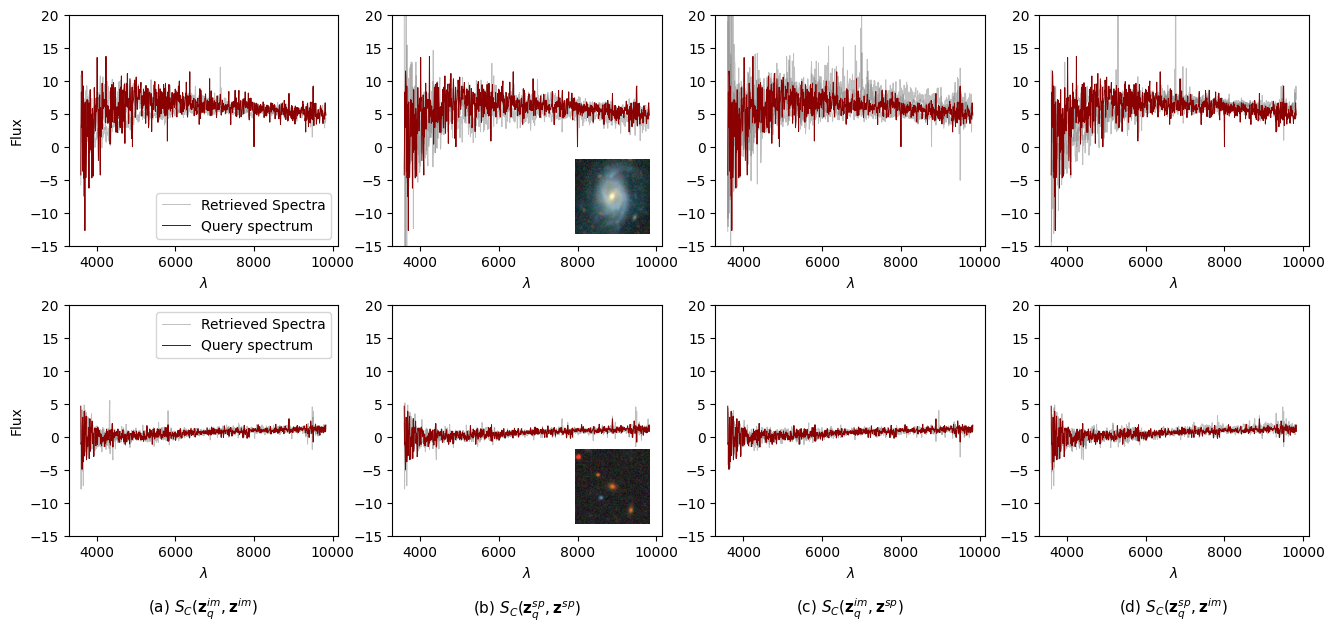
\includegraphics[width=1\textwidth]{figures/sim_search_spectra}}
    \caption{Cosine similarity search for spectra using the 128-dimensional model.
    Each row shows a query galaxy (galaxy imaged in (b)), each subfigure shows the 3 most similar spectra to the query galaxy
       for the given prediction type.}
    \label{fig:sss}
\end{figure}

The best 128-dimensional embedding model was used to perform similarity searches using cosine similarity
(Equation~\eqref{eq:cosine-similarity}) on the learned embeddings.
Unlike ~\cite{stein2021}, our model is not constrained to only performing in-modality image searches and Figures~\eqref{fig:ssia}
and~\eqref{fig:sss} show the results of both in-modal and cross-modal similarity searches for images and spectra respectively.
The results show that the model is able to retrieve similar images and spectra to the query image and spectrum, respectively,
even across modalities.
As described by ~\cite{stein2021}, this ability is critical when searching for rare astronomical sources and the cross-modal
ability of the model adds significantly to this.
